\documentclass[11pt]{beamer}
\usetheme{Berlin}
\usepackage[utf8]{inputenc}
\usepackage[english]{babel}
\usepackage{amsmath}
\usepackage{amsfonts}
\usepackage{amssymb}
\usepackage{graphicx}
\usepackage{hyperref}
\usepackage{listings}
\usepackage{minted}
\usepackage{lipsum}
\usepackage[11pt]{moresize}

\hypersetup{
    colorlinks=true,
    linkcolor=blue,    
    urlcolor=blue
}

\beamertemplatenavigationsymbolsempty
\setbeamertemplate{caption}{\raggedright\insertcaption\par}
\newcommand{\nologo}{\setbeamertemplate{logo}{}}
\newcommand{\reducedfontsizesmall}{\fontsize{10pt}{12}\selectfont}
\newcommand{\reducedfontsizeextrasmall}{\fontsize{8pt}{9.6}\selectfont}

\author{Patrick Nagel}
\title{Java Introduction}
\logo{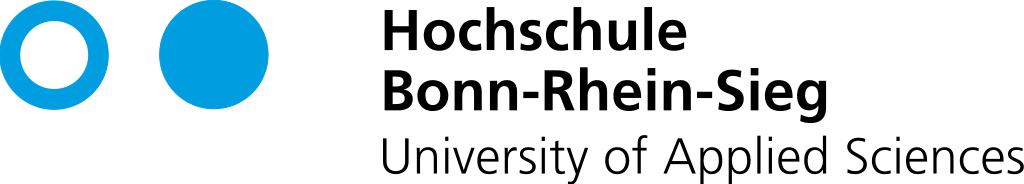
\includegraphics[scale=0.13]{misc/hbrs_logo.png}}
\institute{University of Applied Sciences Bonn-Rhein-Sieg} 
\subject{Foundation Course 2018}

\begin{document}

	\begin{frame}
		\titlepage
	\end{frame}

	\begin{frame}
		\tableofcontents
	\end{frame}

	{\nologo
	\begin{frame}{Java - Yet Another Programming Language}
		\section{Java - Yet Another Programming Language}
		{\reducedfontsizesmall
		Courses in which Java will play a role:
		\begin{itemize}
			\item{Advanced Software Technology.}
			\item{Planning and Scheduling.}
			\item{Multiagent Systems.}
		\end{itemize}
	
		~\\
	
		Advantages of Java in these subjects:
		\begin{itemize}
			\item{Extensive libraries.}
			\item{Elaborated concepts.}
		\end{itemize}
		
		~\\
		
		Further reasons to learn Java:
		\begin{itemize}
			\item{Used in Android development.}
			\item{Avarage salary of a Java developer in Germany: \$53,763 \\(source: \href{https://insights.stackoverflow.com/survey/2017}{stack overflow developer survey results 2017}).}
		\end{itemize}
		}
	\end{frame}
	}

	
	\begin{frame}{Java Basics - Properties}
		\section{Java Basics}
		\subsection{Properties}
		Java is a high-level programming language developed by \textit{Sun Microsystems} an released in 1995.
		~\\
		~\\
		Java is:
		\begin{itemize}
			\item{Object Oriented.}
			\item{Platform Independent.}
			\item{Multithreaded.}
			\item{Interpreted.}
			\item{Dynamic.}
		\end{itemize}
	\end{frame}
	
	{\nologo
	\begin{frame}{Java Basics - How does Java work?}
		\subsection{How does Java work?}
		\begin{columns}[T,onlytextwidth]
			\begin{column}{.4\textwidth}
				\begin{minipage}{\textwidth}
					\begin{itemize}
						\item{High-level language $\neq$ machine code.}
						\item{Compilation and interpretation needed!}
					\end{itemize}
					~\\
					{\reducedfontsizesmall
					The steps in Java are:
					\begin{enumerate}
						\item{Write code in .java file.}
						\item{Compile into Java byte code.}
						\item{Execute byte code with help of Java Virtual Machine (JVM).}
					\end{enumerate}
					}
				\end{minipage}
			\end{column}
			\begin{column}{.4\textwidth}
				\begin{minipage}{\textwidth}
					\begin{figure}
						\centering
						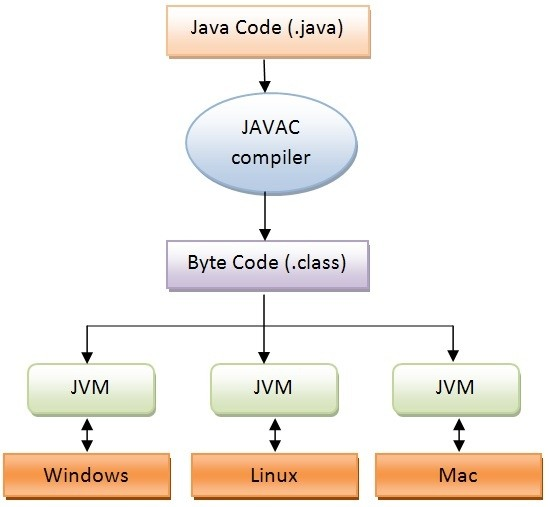
\includegraphics[scale=0.26]{images/how_does_java_work.jpeg}
						\caption{Source: \href{https://www.quora.com/What-is-the-Java-virtual-machine-JVM}{www.quora.com}}
					\end{figure}
				\end{minipage}			
			\end{column}
		\end{columns}
	\end{frame}
	}
	
	{\nologo
	\begin{frame}{Syntax and Further Characteristics}
		\section{Syntax and Further Characteristics}
		{\reducedfontsizeextrasmall
		\begin{itemize}
			\item{Java is \textit{case sensitive} - difference between \textbf{cool} and \textbf{Cool}.}
			\item{Java follows the \textit{CamelCase} convention.}
			\item{Java is a strict data typing language: Every variable must be declared with a data type.}
		\end{itemize}
		\noindent\rule{\textwidth}{0.1pt}
		\begin{itemize}
			\item{Class names start with a capital letter.}
			\item{Method and variable names start with a small letter.}
			\item{Names used for classes, methods and variables are referred to as \textit{identifiers}. For that certain rules exist:}
			\begin{itemize}
				{\reducedfontsizeextrasmall
				\item{All identifiers start with a letter, a currency symbol or an underscore.}
				\item{After the first character identifiers can have any combination of characters.}
				\item{A key word cannot be used as an identifier.}
				}
			\end{itemize}
			\item{Reserved key words may not be used as identifier names. A list of all keywords can be found \href{https://docs.oracle.com/javase/tutorial/java/nutsandbolts/_keywords.html}{here}.}
		\end{itemize}
		}
	\end{frame}
	}
	
	\begin{frame}{Basic Elements - Repetition}
		\section{Basic Elements}
		\subsection{Repetition}
		{\reducedfontsizeextrasmall
		Java programs consist of objects, that communicate via invoking each other's methods.
		
		\begin{itemize}
			\item{\textbf{Comments}: Allow the programmer to make notes inside the code.}
			\item{\textbf{Variables}: The values assigned to the variables define the state of an object or a class.}
			\item{\textbf{Objects}: Have states and behaviors.}
			\item{\textbf{Class}: Blueprint/template of an object. A class describes the behavior and states that the object supports.}
			\item{\textbf{Methods (functions)}: Collections of statements that are grouped together to perform an operation. Methods represent the behavior. A class can contain many methods.}
			\item{\textbf{Decisions}: Structures that have one or more conditions to be evaluated or tested by the program.}
			\item{\textbf{Loops}: Statements that allow to execute a block of code several number of times.}
			\item{\textbf{Input/Output}: Self explaining.}
			\item{...}
		\end{itemize}
		}
	\end{frame}
	
	{\nologo
	\begin{frame}{Basic Elements - Examples in Java (1/3)}
		\subsection{Examples in Java}
		\ssmall \inputminted[firstline=5,lastline=26]{java}{code/BasicElements.java}
	\end{frame}
	}
	
	{\nologo
	\begin{frame}{Basic Elements - Examples in Java (2/3)}
		\ssmall \inputminted[firstline=28,lastline=36]{java}{code/BasicElements.java}
	\end{frame}
	}
	
	{\nologo
	\begin{frame}{Basic Elements - Examples in Java (3/3)}
		\ssmall \inputminted[firstline=38,lastline=59]{java}{code/BasicElements.java}
	\end{frame}
	}
	
	\begin{frame}{Basic Elements - Demo via Terminal}
		\subsection{Demo via Terminal}
		\begin{enumerate}
			\item{Download the file \textit{BasicElements.java} from the repository.\\ {\ssmall \textit{foundation\_cours $>$ content $>$ programming $>$ java\_introduction $>$ code}}}
			\item{Compile the file with the help of the terminal and the command\\ \textbf{javac BasicElements.java}}
			\item{Execute the created byte code with\\ \textbf{java BasicElements $<$argument$>$}}
		\end{enumerate}
	\end{frame}
	
	\begin{frame}{Basic Elements - Challenge}
		\subsection{Challenge}
		Create a class representing a student. The student is suppose to have the following properties:
		\begin{itemize}
			\item{\textit{First name} and \textit{last name}.}
			\item{\textit{Age}.}
			\item{\textit{Favorite subject}.}
		\end{itemize}
		
		Further write a method that prints all the aforementioned information in a sentence.\\
		
		The student is created on runtime and the necessary information are passed via console.\\

		\textbf{Good luck! You have 20mins.}
	\end{frame}
	
	\begin{frame}{Debugging}
		\section{Debugging}
				
		Types of errors:
		\begin{itemize}
			\item{\textbf{Syntactical Errors}: e.g. missing semicolon.}
			\item{\textbf{Logical Errors}: e.g. the method \textit{withdrawMoney()} adds money to the bank account rather than subtracting it.}	
		\end{itemize}
		~\\
		Debugging is the process of finding and resolving defects or problems within a computer program.\\
		
		Eclipse:
		\begin{itemize}
			\item{Shows \textit{syntax errors} right away: 
\includegraphics[scale=0.05]{images/eclipse_error_symbol.jpeg}}
			\item{Provides for \textit{logical errors} a debug tool.}
		\end{itemize}		 
	\end{frame}
	
	\begin{frame}{Object Oriented Principles -Inheritance}
		\section{Object Oriented Principles}
		\subsection{Inheritance}
		Inheritance can be defined as the process where one class acquires the properties (methods and fields) of another. With the help of inheritance information are managed in a hierarchical manner.\\
		
		Example: 
		\begin{columns}[T,onlytextwidth]
			\begin{column}{.4\textwidth}
				\begin{minipage}{\textwidth}
					\ssmall \inputminted[firstline=3,lastline=9]{java}{code/Parent.java}
				\end{minipage}
			\end{column}
			\begin{column}{.4\textwidth}
				\begin{minipage}{\textwidth}
					\ssmall\inputminted[firstline=3,lastline=9]{java}{code/Child.java}
				\end{minipage}			
			\end{column}
		\end{columns}
		
		What does that mean? Among other:
		\begin{itemize}
			\item{Child inherits all properties and skills.}
			\item{Redundancies can be avoided.}
		\end{itemize}
	\end{frame}
	
	\begin{frame}{Object Oriented Principles - Abstract Classes}
		\subsection{Abstract Classes}
		Abstract classes represent classes that cannot be instantiated. However other classes can inherit from abstract classes and then be instantiated with the properties of the abstract class. It is used as a process of hiding the implementation from the user.\\
		
		Facts about abstract classes:
		\begin{itemize}
			\item{Contain the word \textit{abstract} in their declaration.}
			\item{May or may not contain \textit{abstract methods}(=methods whose body still needs to be defined by the heirs).}
			\item{If a class has at least one abstract method it needs to be declared bastract.}
		\end{itemize}
	\end{frame}	
	
	\begin{frame}{Object Oriented Principles - Interfaces}
		\subsection{Interfaces}
		An interface in Java is a collection of constants and abstract methods. A class implements an interface, thereby inheriting the abstract methods of the interface.\\
		
		Facts about interfaces:
		\begin{itemize}
			\item{A class can implement more than one interface.}
			\item{Similar to abstract classes, an interface cannot be instantiated.}
			\item{Interfaces do not contain any constructors.}
			\item{Fields in interfaces can only be declared both \textit{static} and \textit{final}.}
			\item{An interface can extend multiple interfaces.}
		\end{itemize}
	\end{frame}

	\begin{frame}{Object Oriented Principles - Challenge}
		\subsection{Challenge}
		Create five classes. Four classes that represent mathematical shapes, namely:
		\begin{itemize}
			\item{Square.}
			\item{Rectangle.}
			\item{Parallelogram.}
			\item{Kite.}
		\end{itemize}
		
		Include methods to compute the area and circumferance of each of the shapes.\\
		 
		One class that contains the main method and outputs the paramters, areas and circumferances of each object.\\
		
		\textbf{Good luck! You have 30mins.}
	\end{frame}
	
\end{document}